\section{Transportation Routes}

\noindent \href{https://nebraskalegislature.gov/laws/statutes.php?statute=19-903}{NRS \S 19-903(2)} requires a comprehensive development to include:

\begin{quote}
    The general location, character, and extent of existing and proposed major roads, streets, and highways, and air and other transportation routes and facilities.
\end{quote}

% \subsection{Surface Transportation Routes}

\noindent Bloomfield has two major roads: Broadway Street traverses north and south, while Highway 84 traverses east and west. Residents have differing assessments of the condition of these streets (refer to \textbf{Figure~\ref{fig:scoreStreets}}): the quality of Broadway Street is in rough shape, but Highway 84 is generally fine.

\begin{figure}[H]
\centering
\begin{framed}
    \caption{Condition of Specific Streets in Bloomfield}
    \label{fig:scoreStreets}
    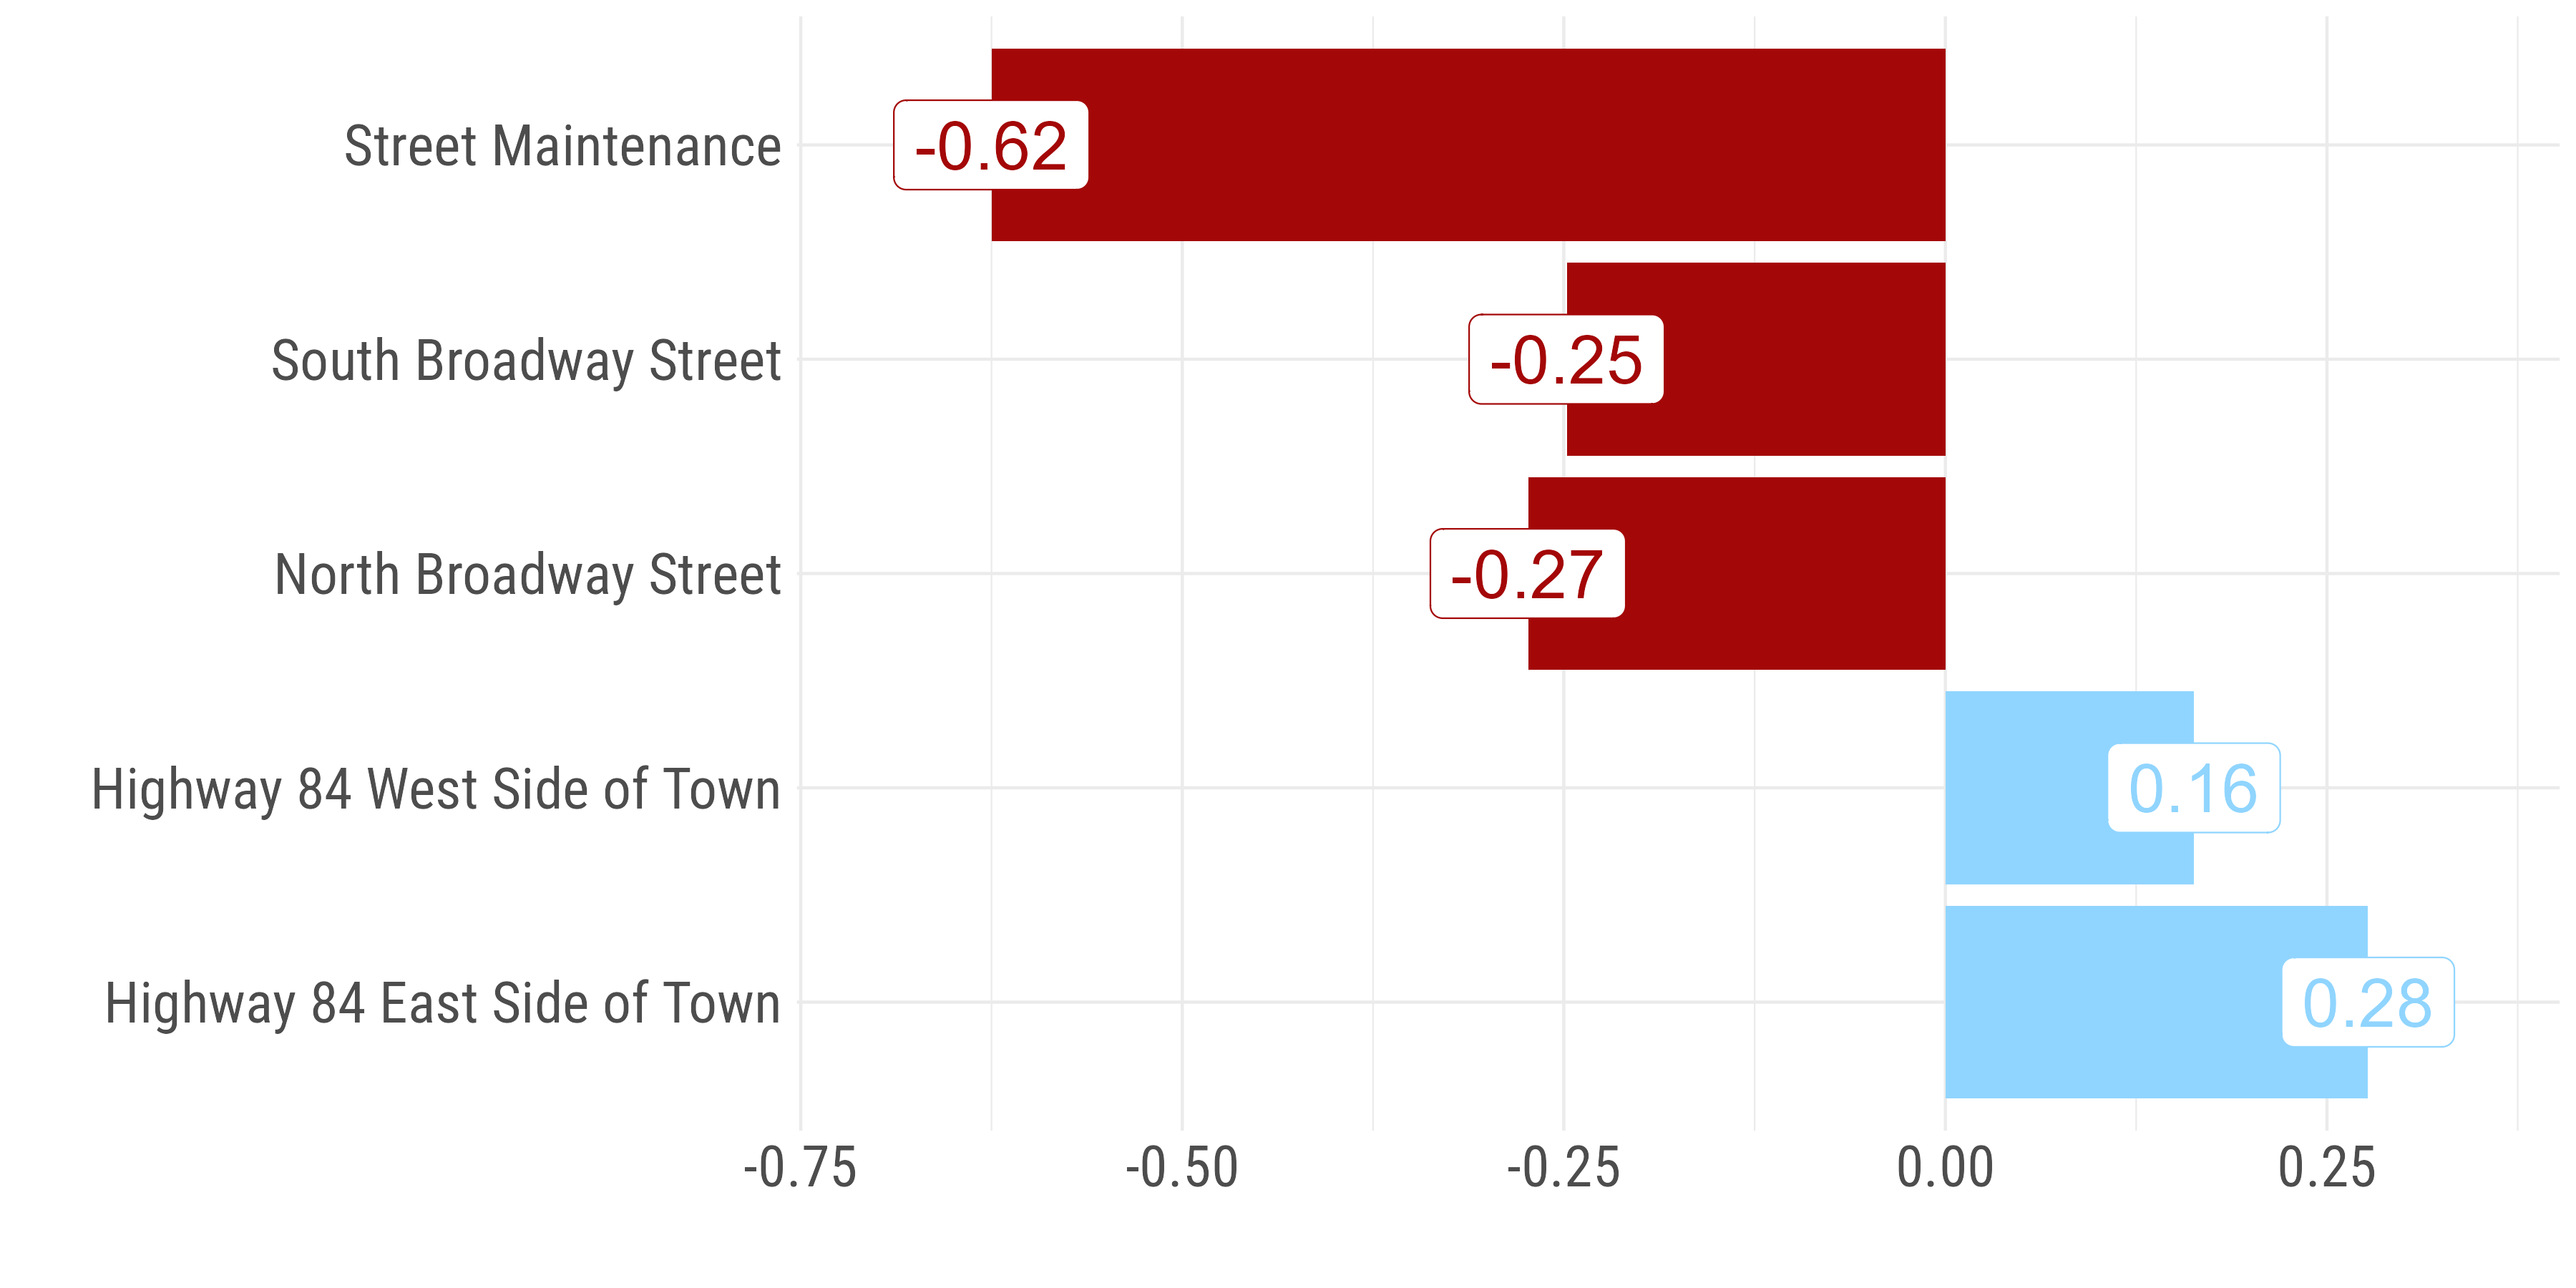
\includegraphics[width = \linewidth]{figures/score_streets.png}
\end{framed}
\end{figure}

\pagebreak
\noindent Moreover, community assessment of streets and sidewalks throughout Bloomfield is generally negative, as \textbf{Figure~\ref{fig:scoreStreetsGeneral}} shows.

\begin{figure}[H]
\centering
\begin{framed}
    \caption{Condition of General Streets and Sidewalks}
    \label{fig:scoreStreetsGeneral}
    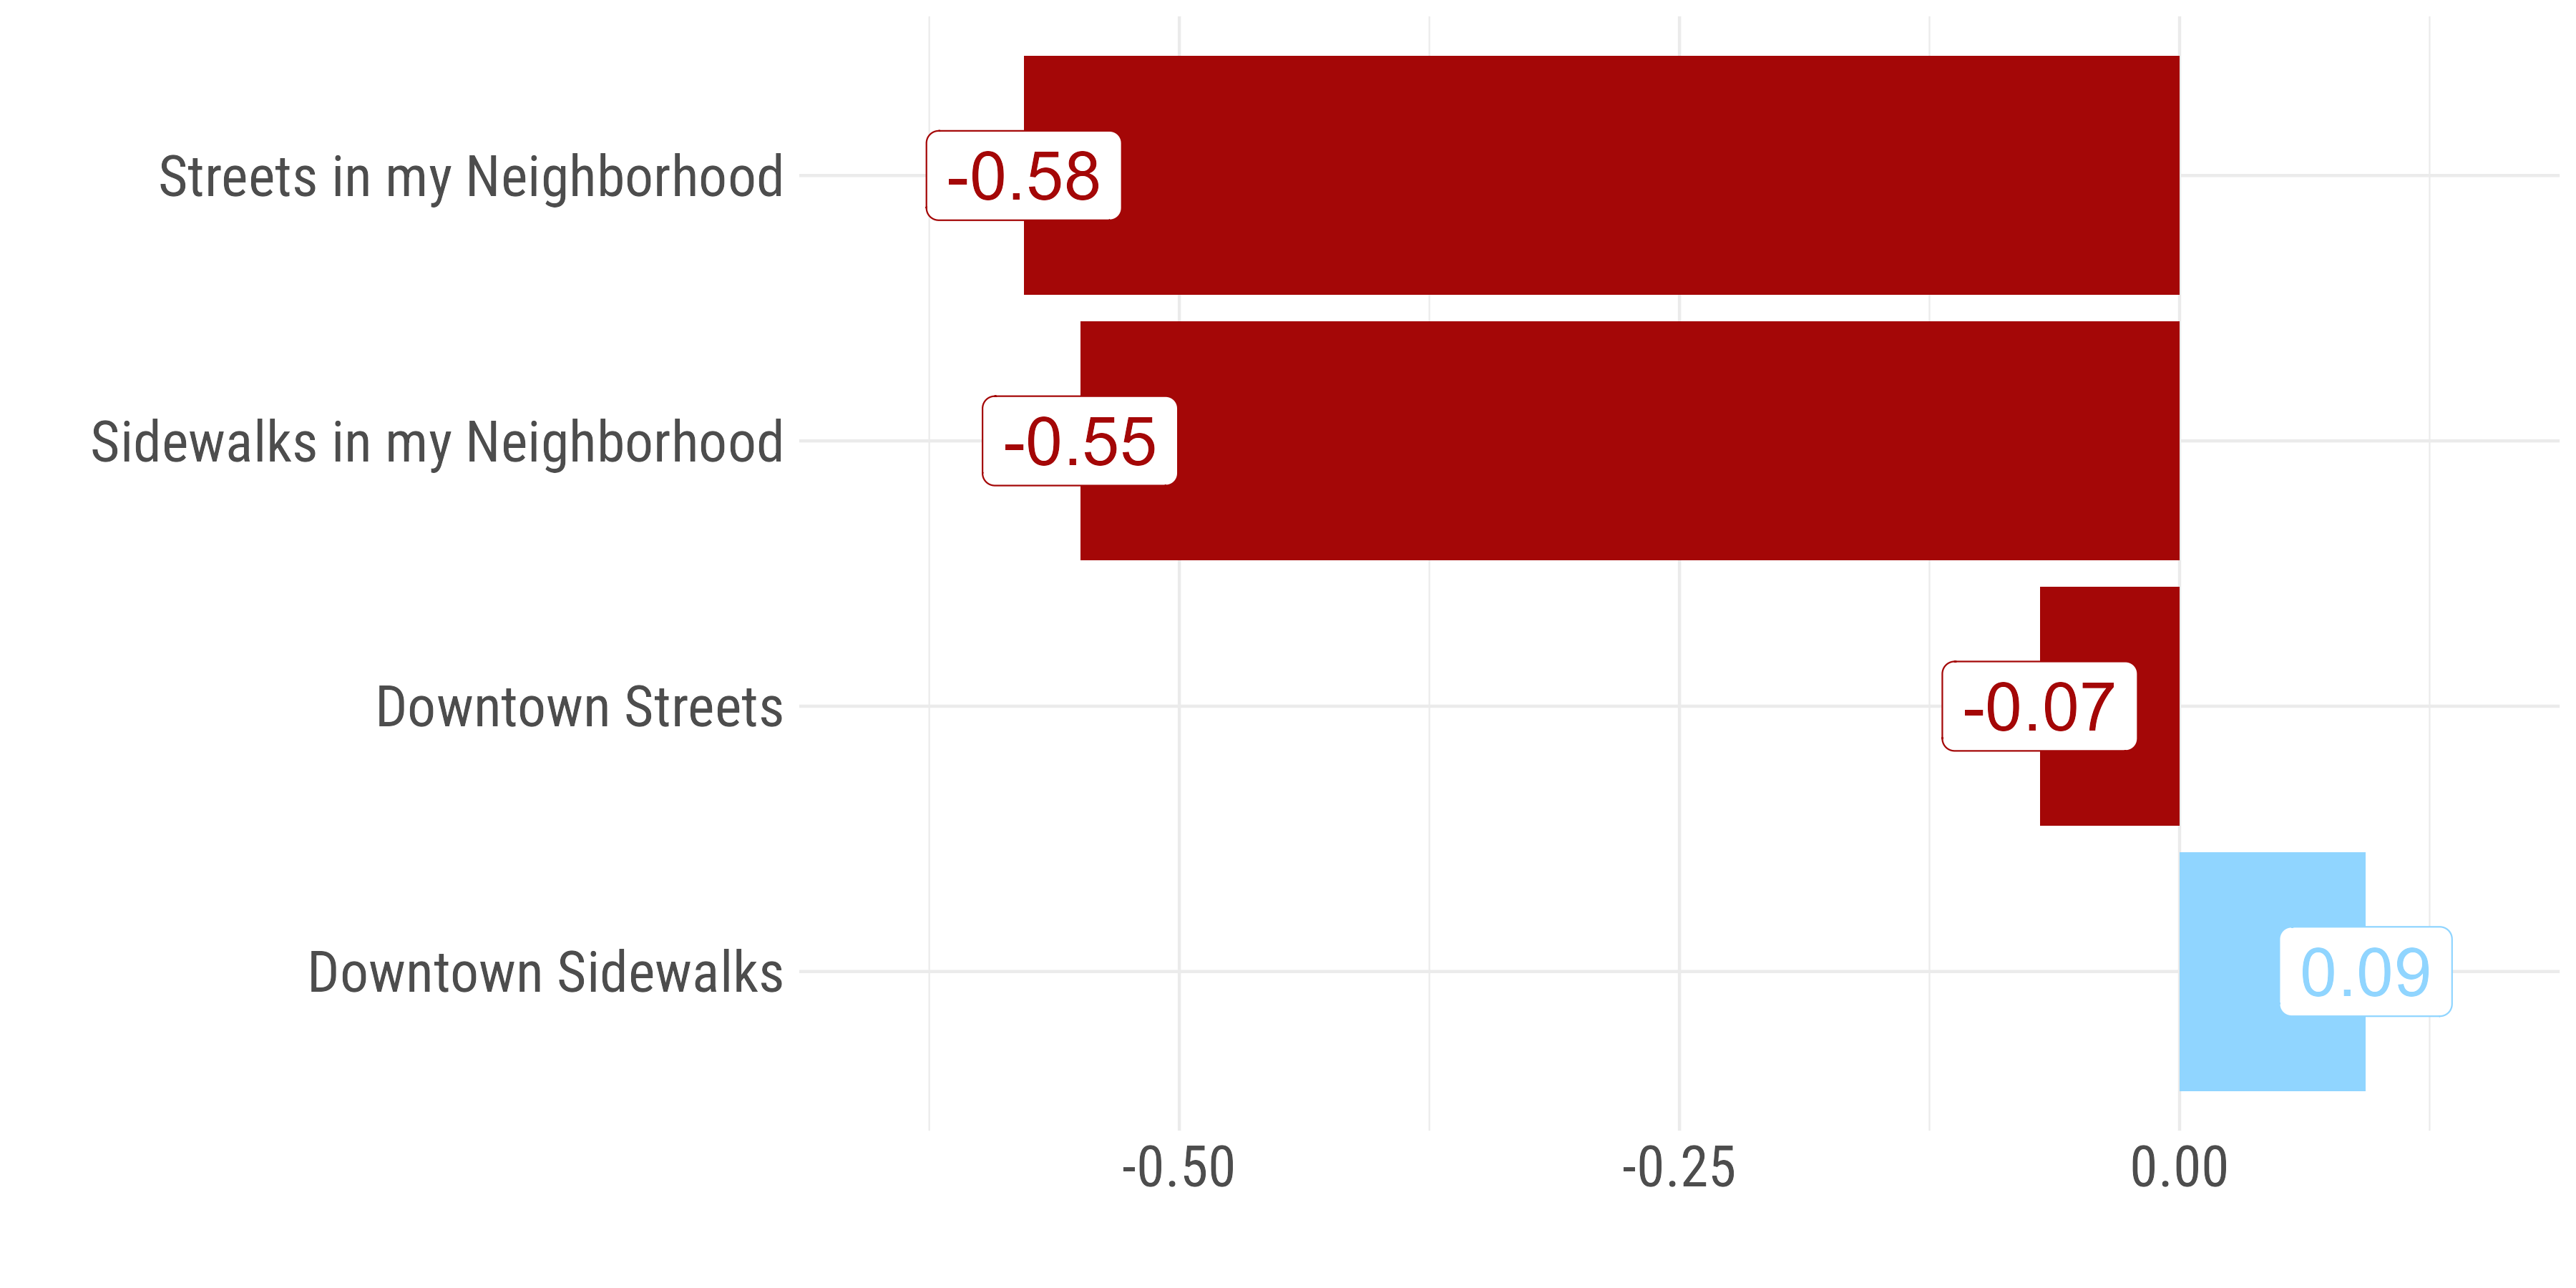
\includegraphics[width = \linewidth]{figures/score_streets_general.png}
\end{framed}
\end{figure}

\noindent Five Rule Rural Planning assessed street conditions in Bloomfield in \hl{[when??]}, creating a map of street conditions in Bloomfield. Our assessment of street conditions off Broadway Street and Highway 84 is similar: we assess that most of the streets in town are in need of some repair, although many of the roads in the southern half of town are in good condition.\\

\noindent In addition, we assessed sidewalk conditions in Bloomfield. Our assessment is similar to the residents'. Downtown sidewalks, near the intersection of Broadway Street and Highway 84, are mostly in good shape. However, Bloomfield residents gave a strong negative rating to sidewalks in their neighborhoods; our assessment is that this is because many neighborhoods do not have sidewalks at all, particularly in the southern half of Bloomfield.\\

\noindent We present our maps of Bloomfield's street and sidewalk conditions on the following pages.

\pagebreak
\thispagestyle{empty}
\begin{landscape}
    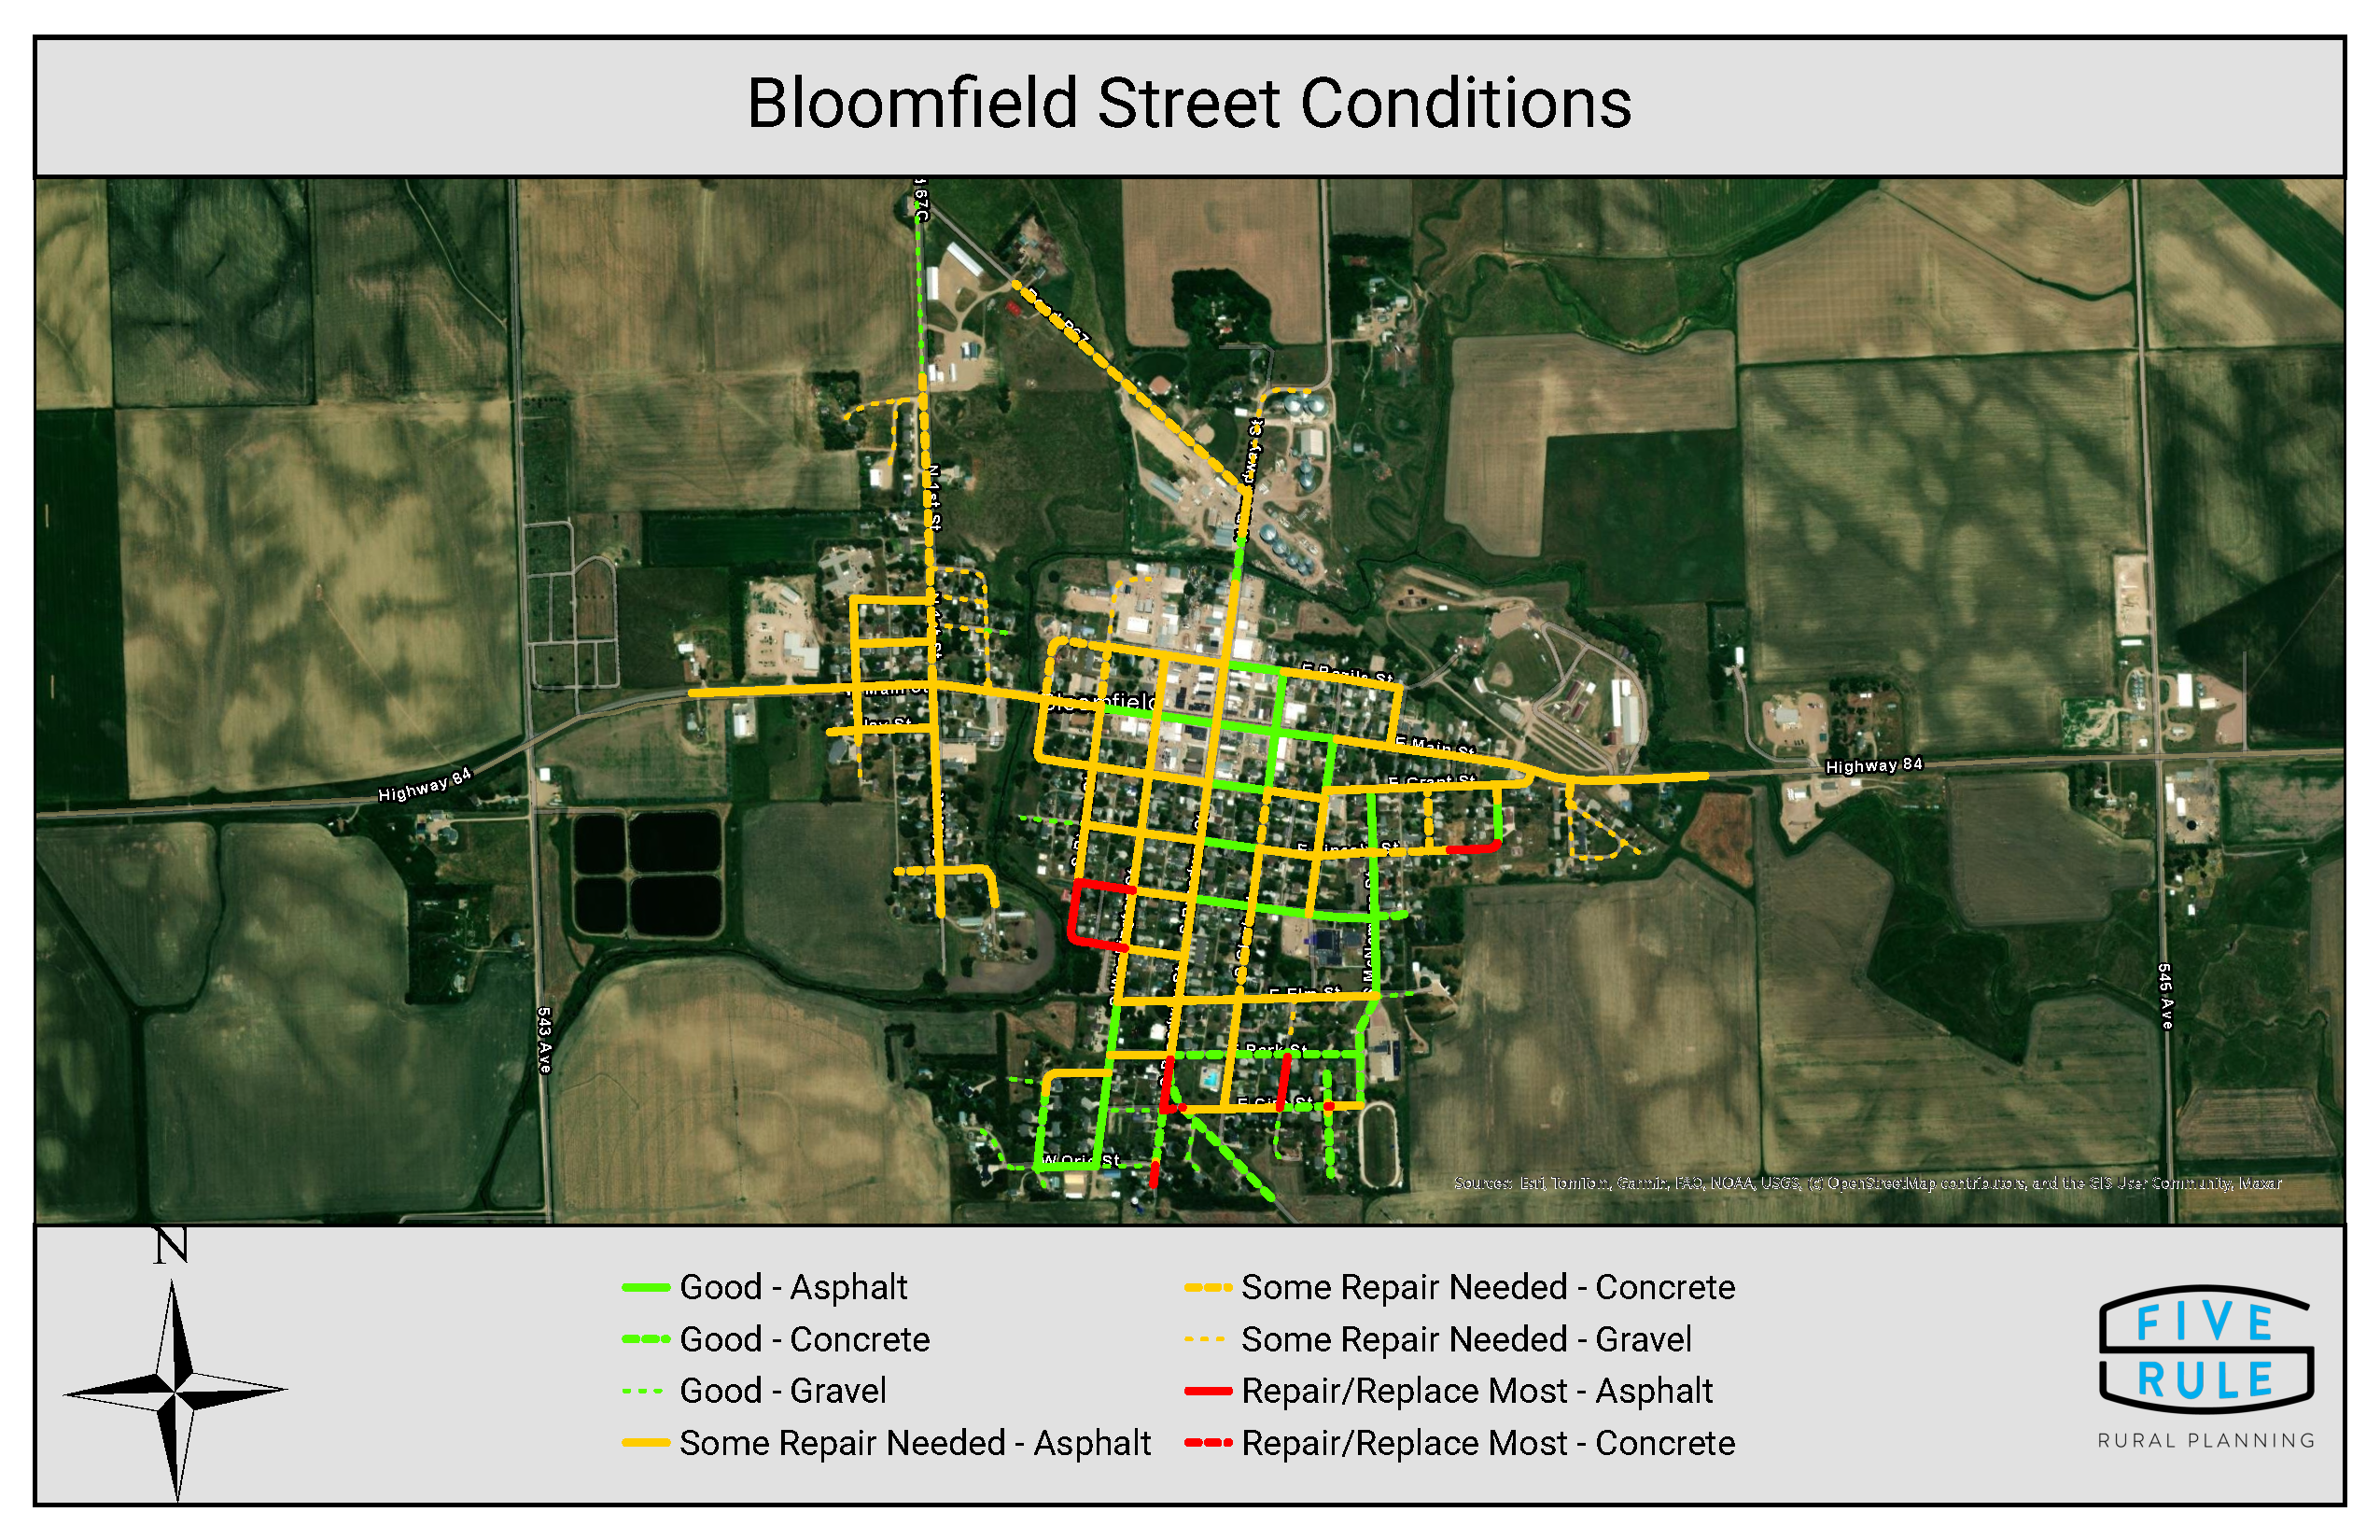
\includepdf[angle = 90]{maps/street_conditions.pdf}
\end{landscape}
\pagebreak

\pagebreak
\thispagestyle{empty}
\begin{landscape}
    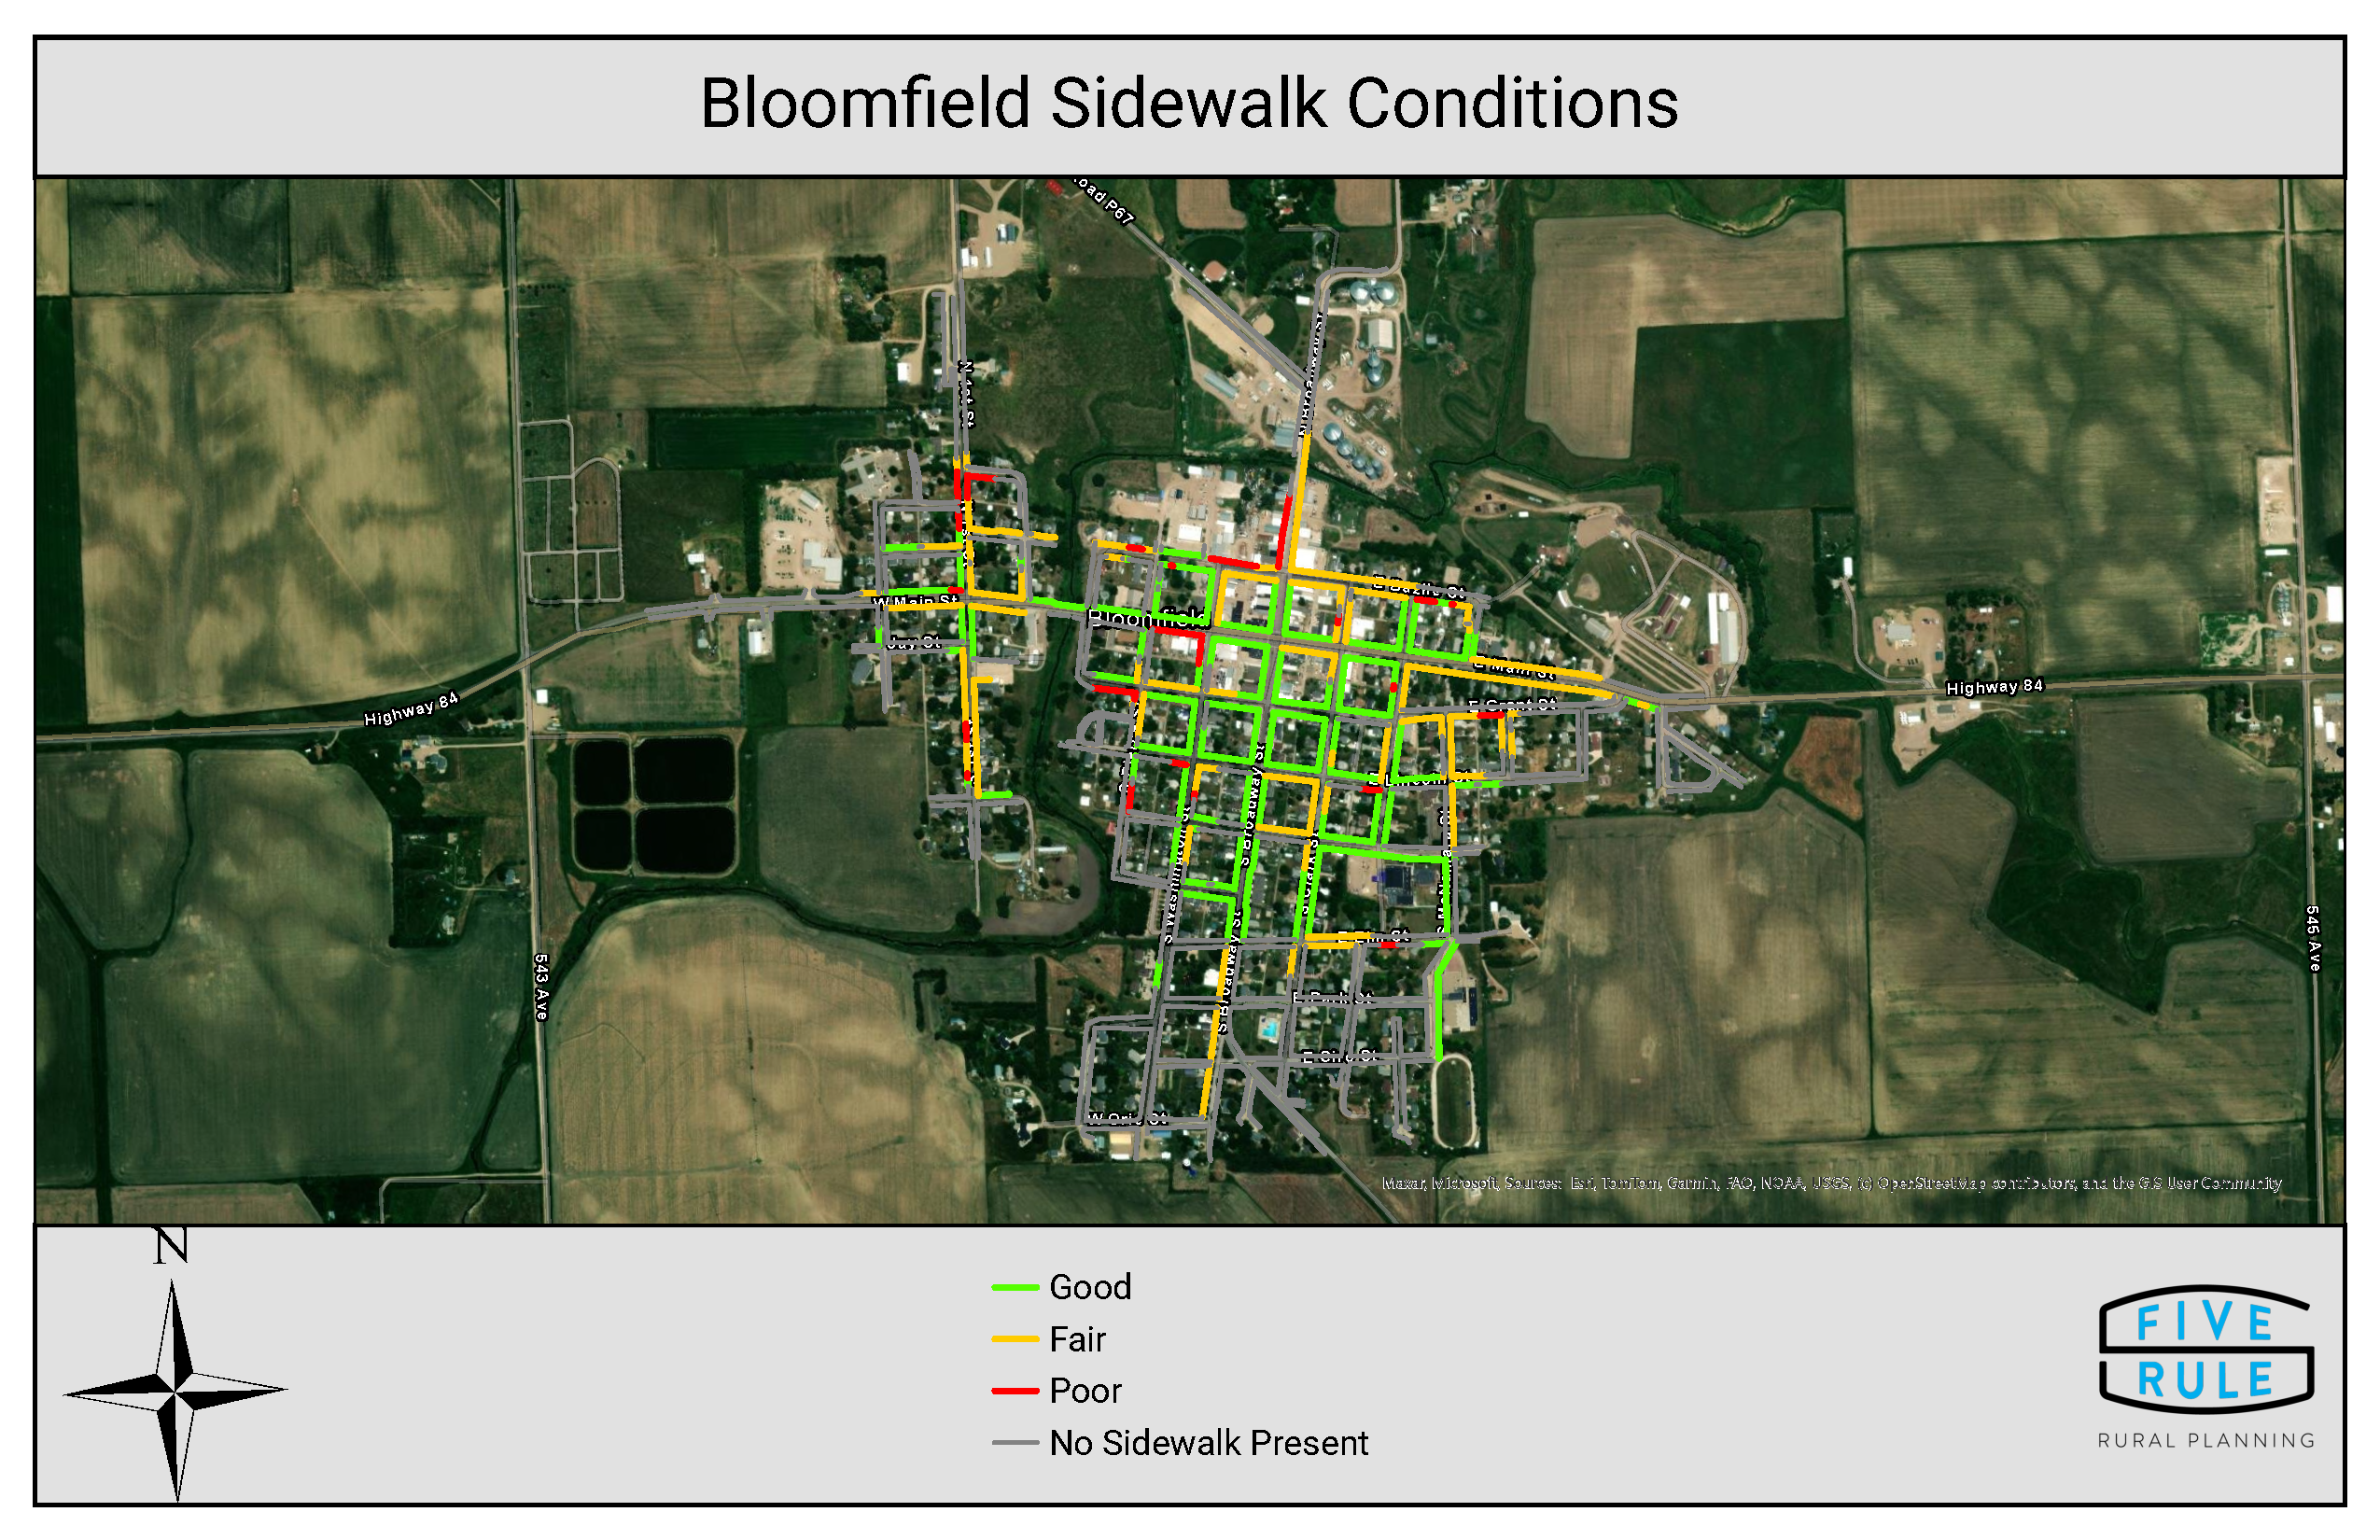
\includepdf[angle = 90]{maps/sidewalk_conditions.pdf}
\end{landscape}
\pagebreak

\subsection*{Key Takeaways}